\begin{surferIntroPage}{Упутство за коришћење}{tutorial_koord1}{Први кораци са SURFER-ом}
%\pdfbookmark{Први кораци са SURFER-ом}{testest}
Овај програм се зове SURFER. Када прочитате ову реч вероватно помислите на воду, сунце и таласе. Но, у овом случају име потиче од речи за површ {\it (на енглеском surface)}.
\\
Помоћу овог програма се могу представити површи, прецизније речено алгебарске површи. Шта ово значи и шта су алгебарске површи је објашњено у овом упутству. Изаберите једну од површи са десне стране да бисте прошли кроз поглавља овог упутства.\\
SURFER је део путујуће изложбе IMAGINARY, која је настала током немачке године математике 2008. Изложба је пројекат интернационално познатог Института за математичка истраживања у Оберволфаху, који се налази на Шварцвалду. Сваке недеље се на том институту одржавају радионице посвећене новијој области математичког истраживања. Ове радионице су значајне јер поспешују размену међу научницима у свету.  \\
\vspace{0.2cm} \hspace{3.5cm}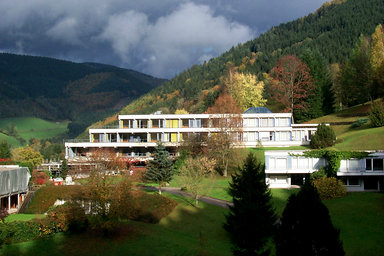
\includegraphics[width=3cm]{./../../common/images/photo_mfo.jpg}\\
SURFER програм се може  бесплатно преузети са странице : \\
\begin{centering}
www.imaginary-exhibition.com\\
\end{centering}
 \vspace{0.2cm}
Са десне стране можете изабрати неко од математичких упутстава, почевши од површи Лимун. Са леве стране можете да одете до других галерија, на пример у галерију површи маште.
\end{surferIntroPage}
